% Jason Wang

A CMOS inverter and CMOS logic NAND gate is constructed to be used in the D Latch layout design.

The width and length of the NMOS to be used in the inverter is given to be $0.5$ \si{\nano\meter} and $0.1$ \si{\nano\meter}, respectively.
The PMOS to be used in the inverter is then designed so that the inverter is matched (steepest slope of the VTC curve occurs when $V_{out} = V_{in} = \frac{V_{DD}}{2}$).
The CMOS inverter is matched using a PMOS with a width $W = 1.2$ \si{\nano\meter} and a length $L = 0.1$ \si{\nano\meter}.
This results in the following layout for the CMOS inverter.

\FloatBarrier

\begin{figure}[h!]
	\centering
	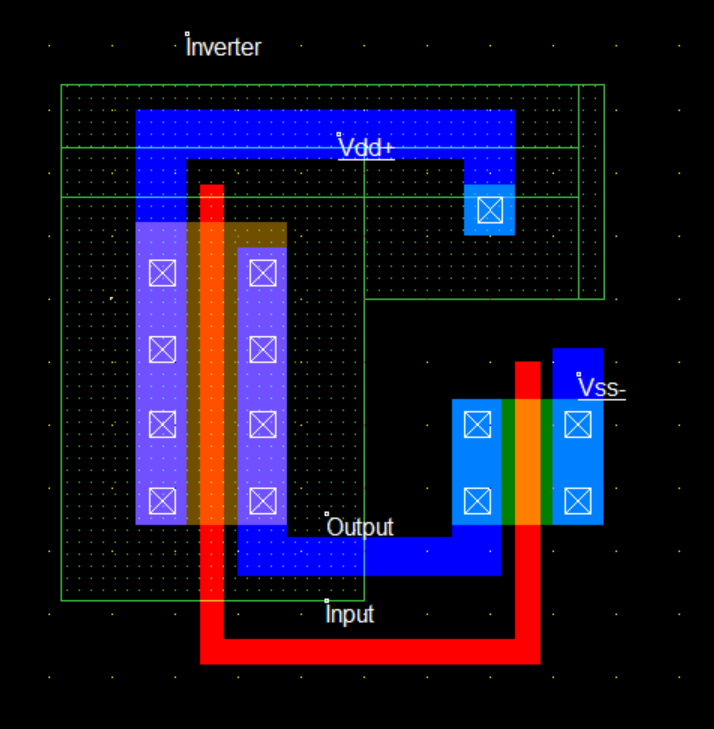
\includegraphics[scale=0.40]{../images/inverter_layout.PNG}
	\caption{CMOS Inverter Layout}
	\label{fig:inverter_layout}
\end{figure}

\FloatBarrier

The VTC of the CMOS inverter shown below verifies that it is matched.

\FloatBarrier

\begin{figure}[h!]
	\centering
	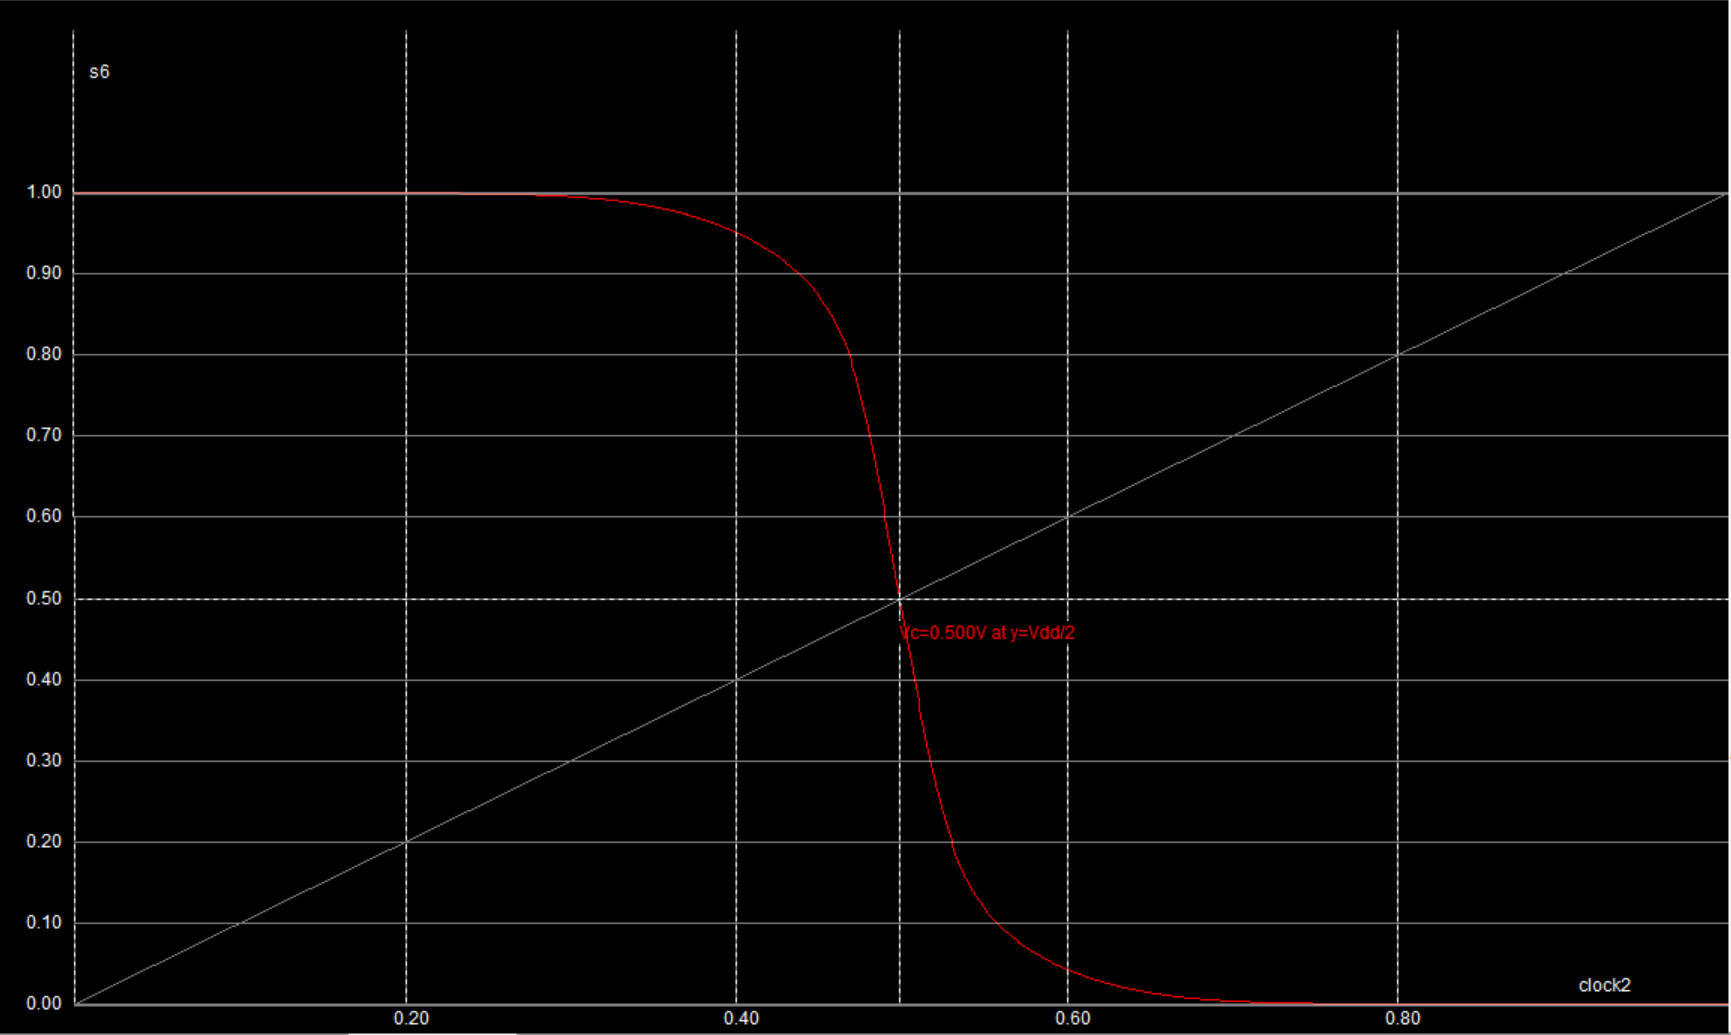
\includegraphics[scale=0.30]{../images/inverter_layout_vtc.PNG}
	\caption{VTC of CMOS Inverter Layout}
	\label{fig:inverter_layout_vtc}
\end{figure}

\FloatBarrier

The logic of the CMOS inverter is verified using a $250$ \si{\mega\hertz} clock input with a rise and fall time of $0.050$ \si{\nano\second}.

\FloatBarrier

\begin{figure}[h!]
	\centering
	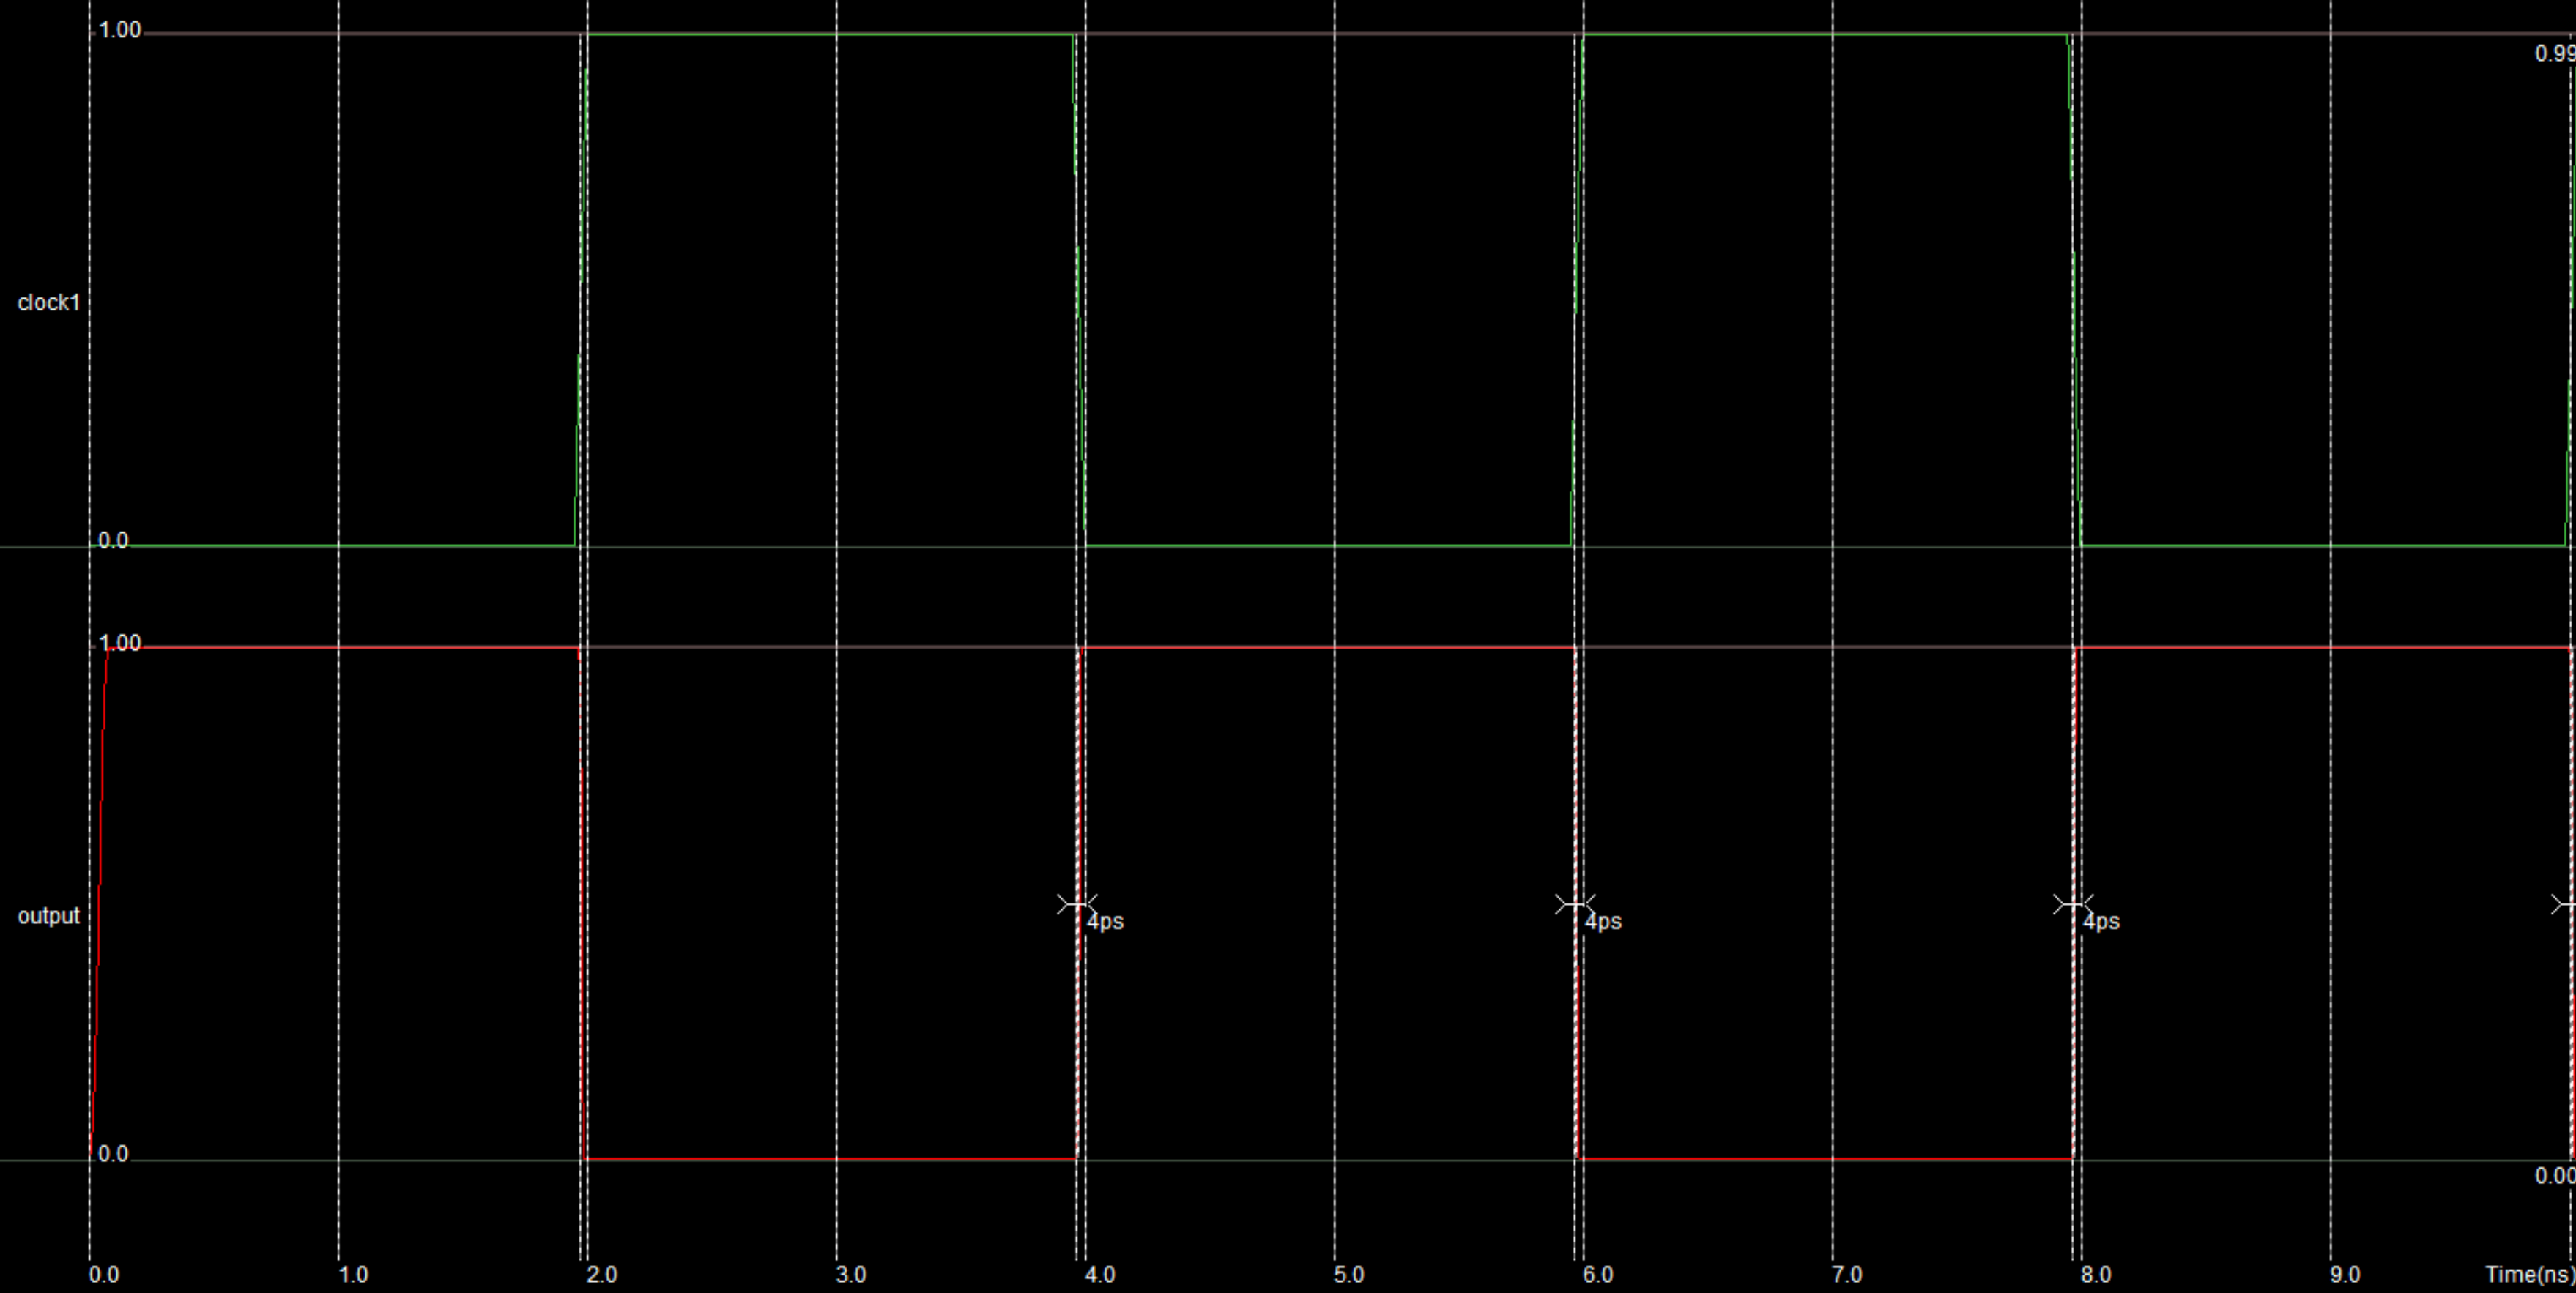
\includegraphics[scale=0.30]{../images/inverter_logic_test.PNG}
	\caption{CMOS Inverter Logic Test}
	\label{fig:inverter_layout_logic}
\end{figure}

\FloatBarrier

Next, a CMOS logic NAND gate is constructed with two PMOS in parallel and two NMOS in series.
The NAND gate is designed so that it operates with the same speed of the CMOS inverter.
To achieve this design goal, the width of both NMOS are doubled to $W = 1.0$ \si{\nano\meter} so that it operates twice as fast to compensate for the speed lost due to having two NMOS connected in series.
This results in the following layout for the NAND gate.

\FloatBarrier

\begin{figure}[h!]
	\centering
	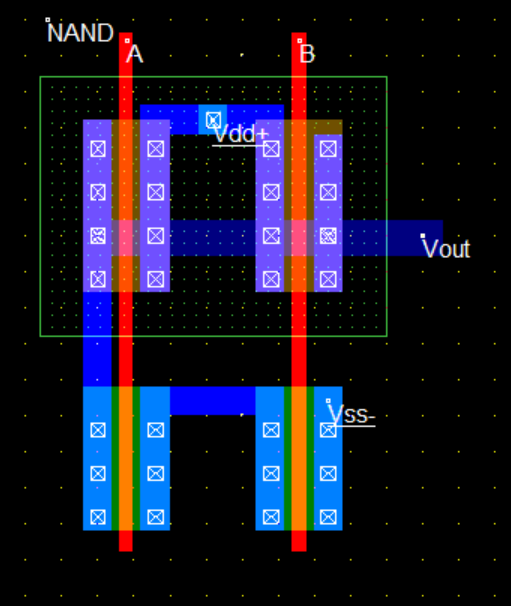
\includegraphics[scale=0.70]{../images/nand_layout.PNG}
	\caption{NAND Gate Layout}
	\label{fig:nand_layout}
\end{figure}

\FloatBarrier

The logic of the NAND gate verified using a $250$ \si{\mega\hertz} clock input and a $125$ \si{\mega\hertz} clock input with rise and fall times of $0.050$ \si{\nano\second}.

\FloatBarrier

\begin{figure}[h!]
	\centering
	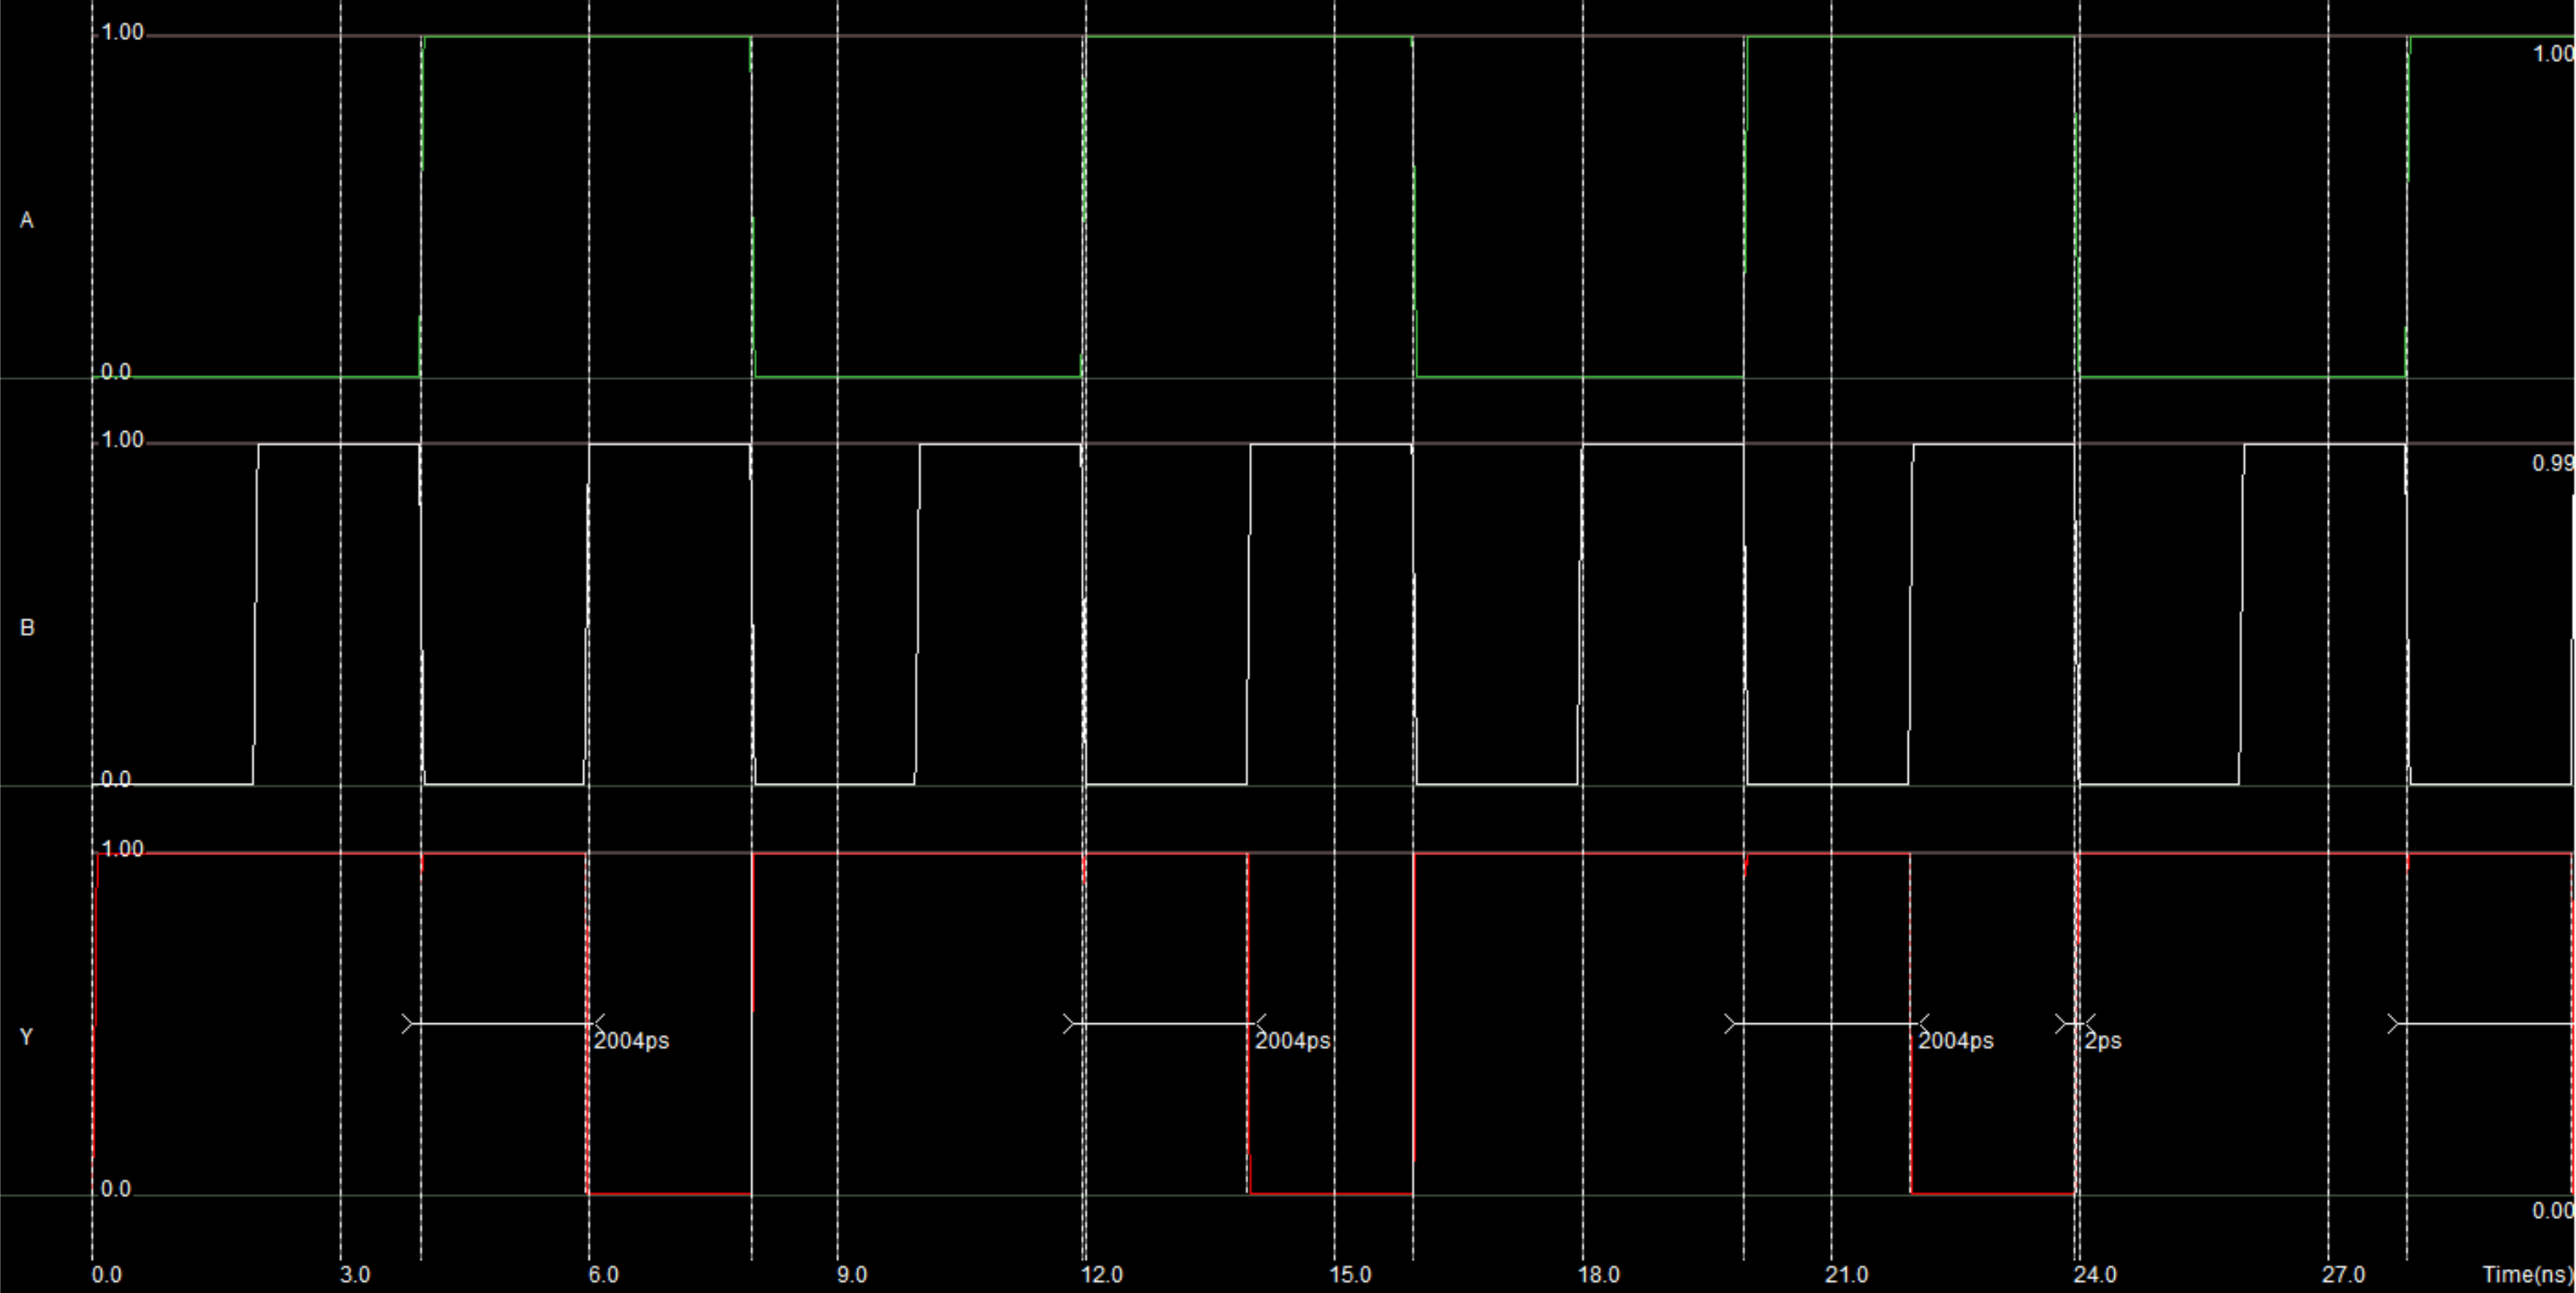
\includegraphics[scale=0.30]{../images/nand_logic_test.PNG}
	\caption{NAND Gate Logic Test}
	\label{fig:inverter_layout_vtc}
\end{figure}

\FloatBarrier

Using the CMOS inverter and NAND gate designed above, the following D Latch layout is constructed.

\FloatBarrier

\begin{figure}[h!]
	\centering
	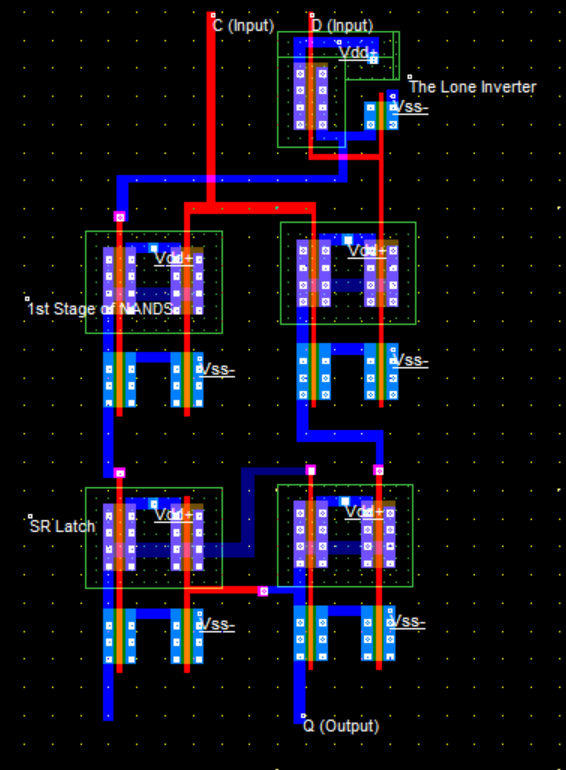
\includegraphics[scale=0.70]{../images/dlatch_layout.PNG}
	\caption{D Latch Layout}
	\label{fig:dlatch_layout}
\end{figure}

\FloatBarrier

The expected behavior of the D Latch can be expressed in the following truth table.

\FloatBarrier

\begin{table}[h!]
	\centering
	\caption{Logic Chart of D Latch Circuit}
	\label{tab:dlatch_logic}
	\csvautotabular{../data/dlatch_logic.csv}
\end{table}

\FloatBarrier

The truth table above translates to the the following finite state machine (FSM).

\FloatBarrier

\begin{figure}[h!]
	\centering
	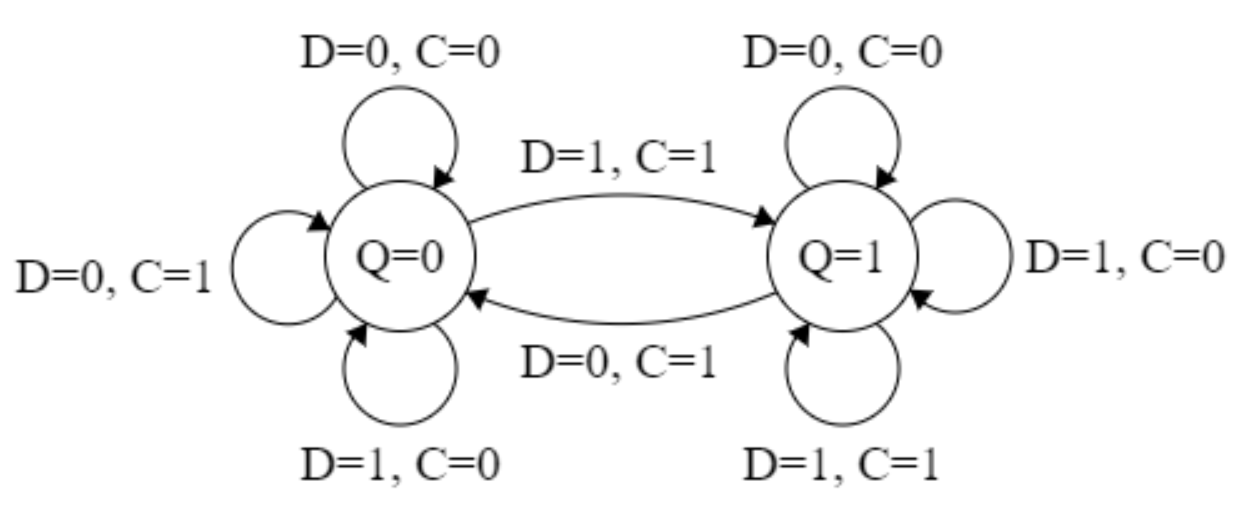
\includegraphics[scale=0.70]{../images/dlatch_fsm.PNG}
	\caption{D Latch FSM}
	\label{fig:dlatch_fsm}
\end{figure}

\FloatBarrier

The delays for the transitions between Q high and Q low ($\tau_{PHL}$) and vise versa ($\tau_{PLH}$) can be used to determine the maximum operating frequency of the D Latch.

The D Latch is tested with input clock C at $250$ \si{\mega\hertz}, $1$ \si{\giga\hertz}, and $4$ \si{\giga\hertz} with clock D always set to half the frequency of C.
Rise and fall times of $0.050$ \si{\nano\second} and $0.001$ \si{\nano\second} are tested for each clock frequency.

\FloatBarrier

\begin{figure}[h!]
	\centering
	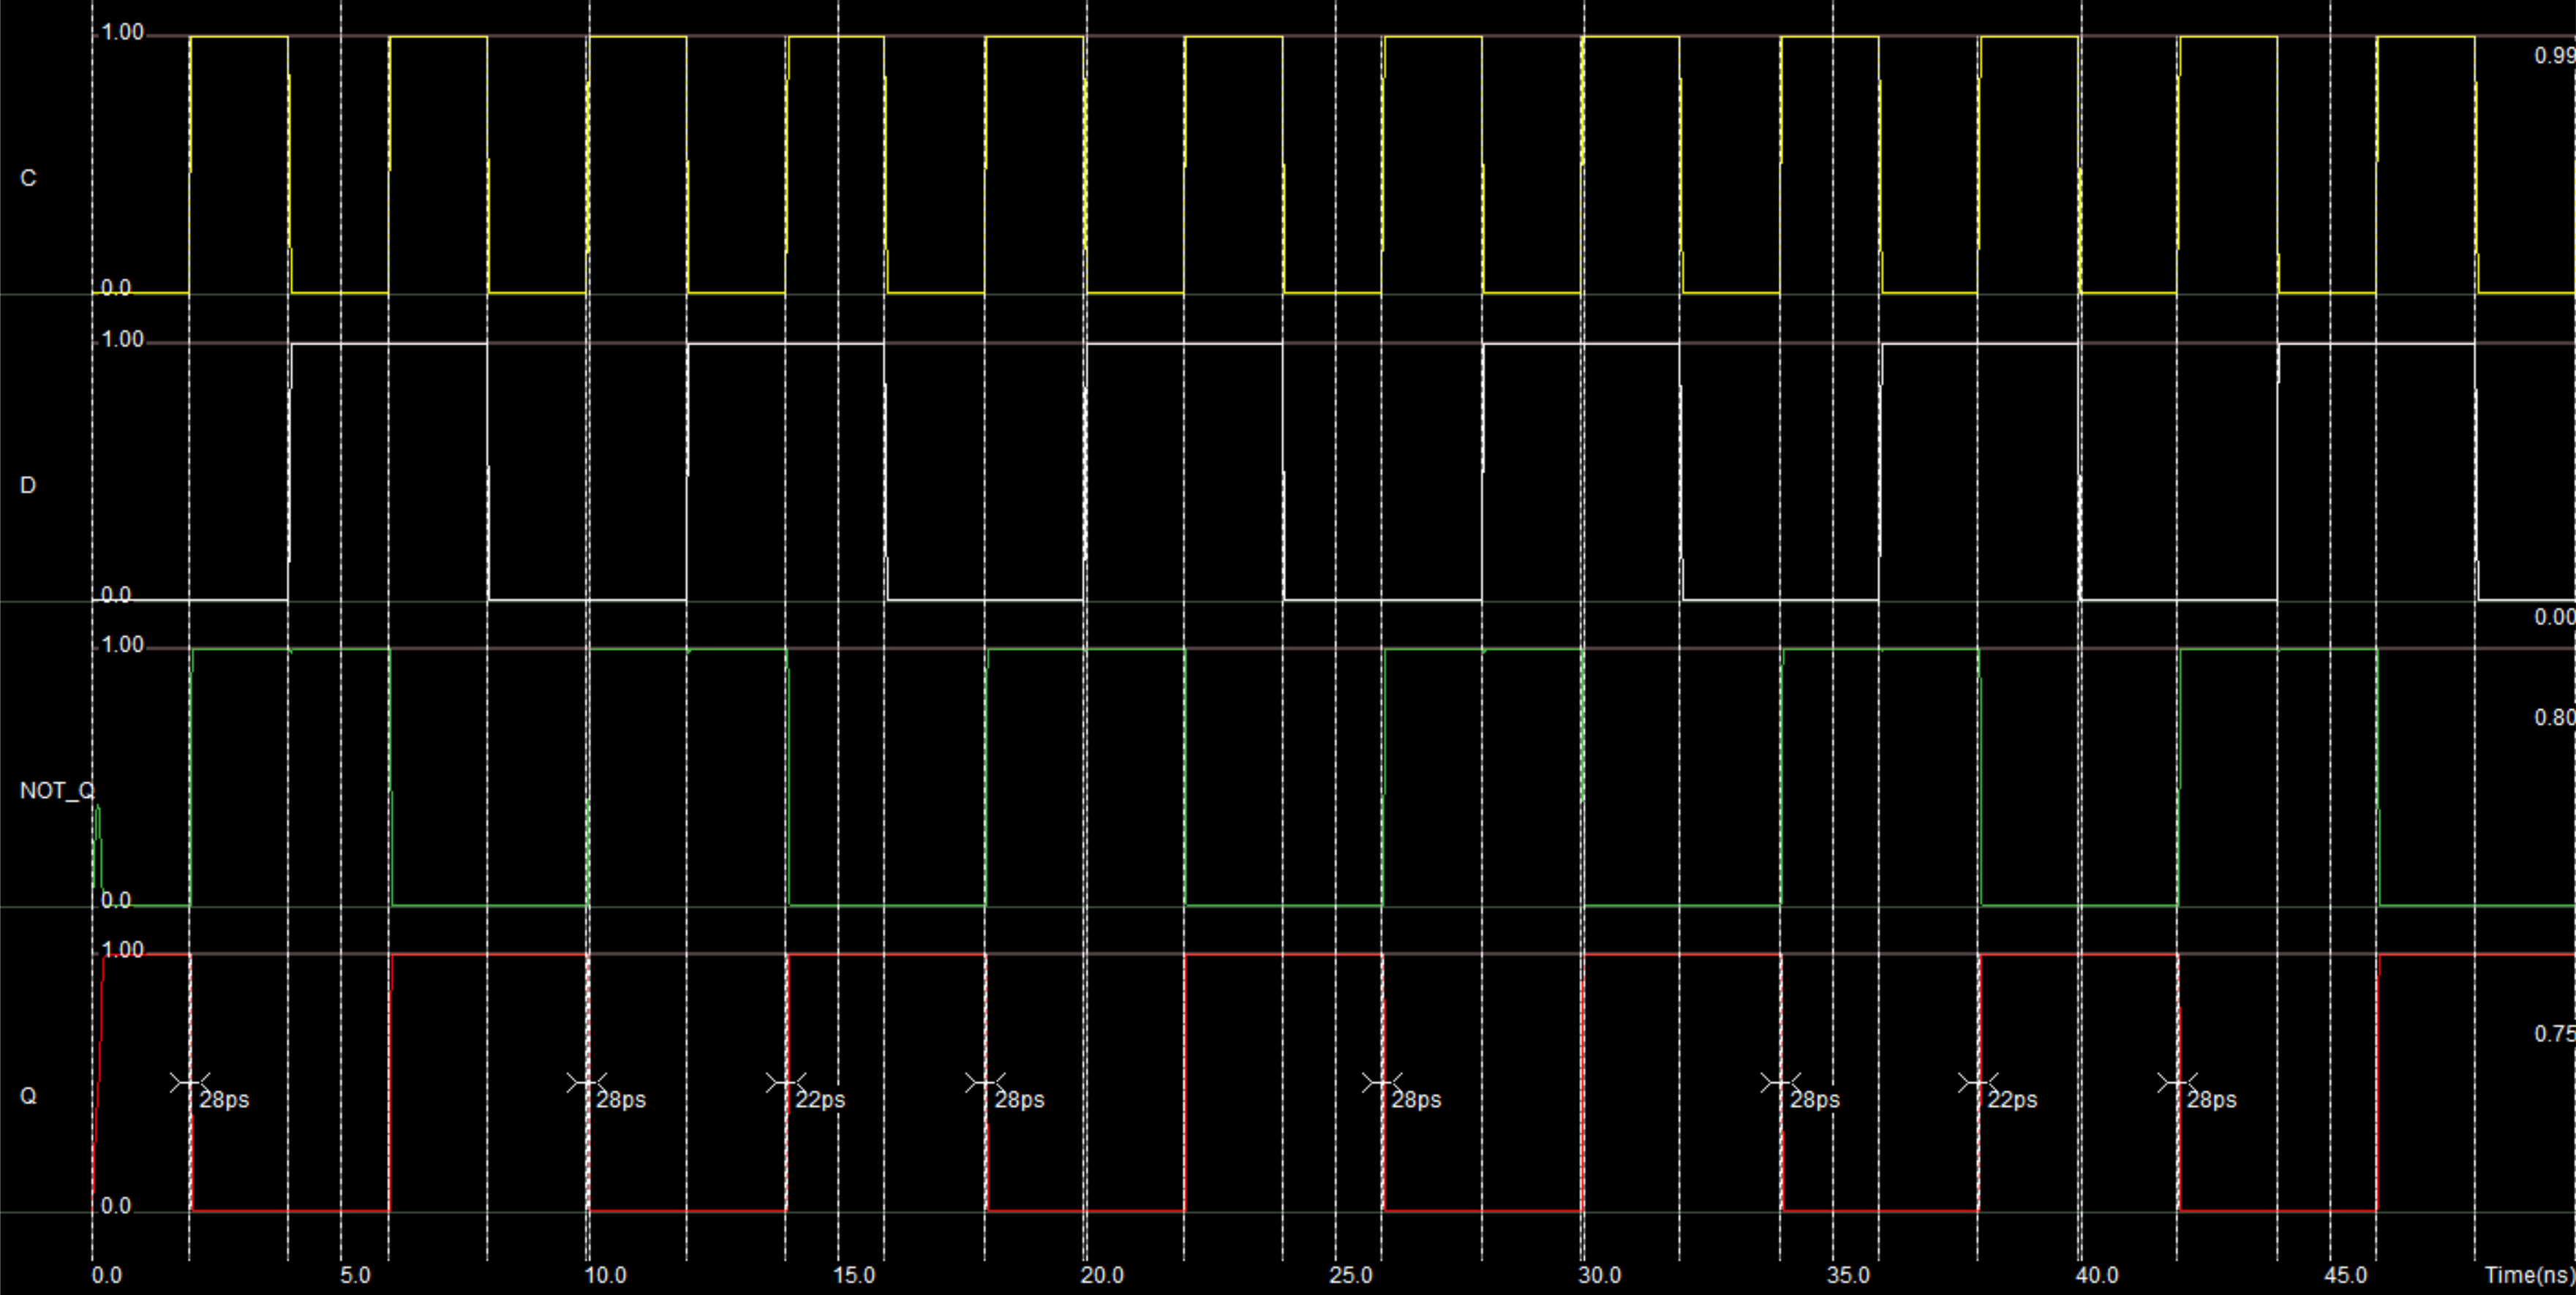
\includegraphics[scale=0.30]{../images/test_inputs_from_manual.PNG}
	\caption{Test Case 1 - $f_C = 250$ \si{\mega\hertz}, Rise/Fall Time $= 0.050$ \si{\nano\second}}
	\label{fig:layout_test_1}
\end{figure}

\FloatBarrier

\begin{figure}[h!]
	\centering
	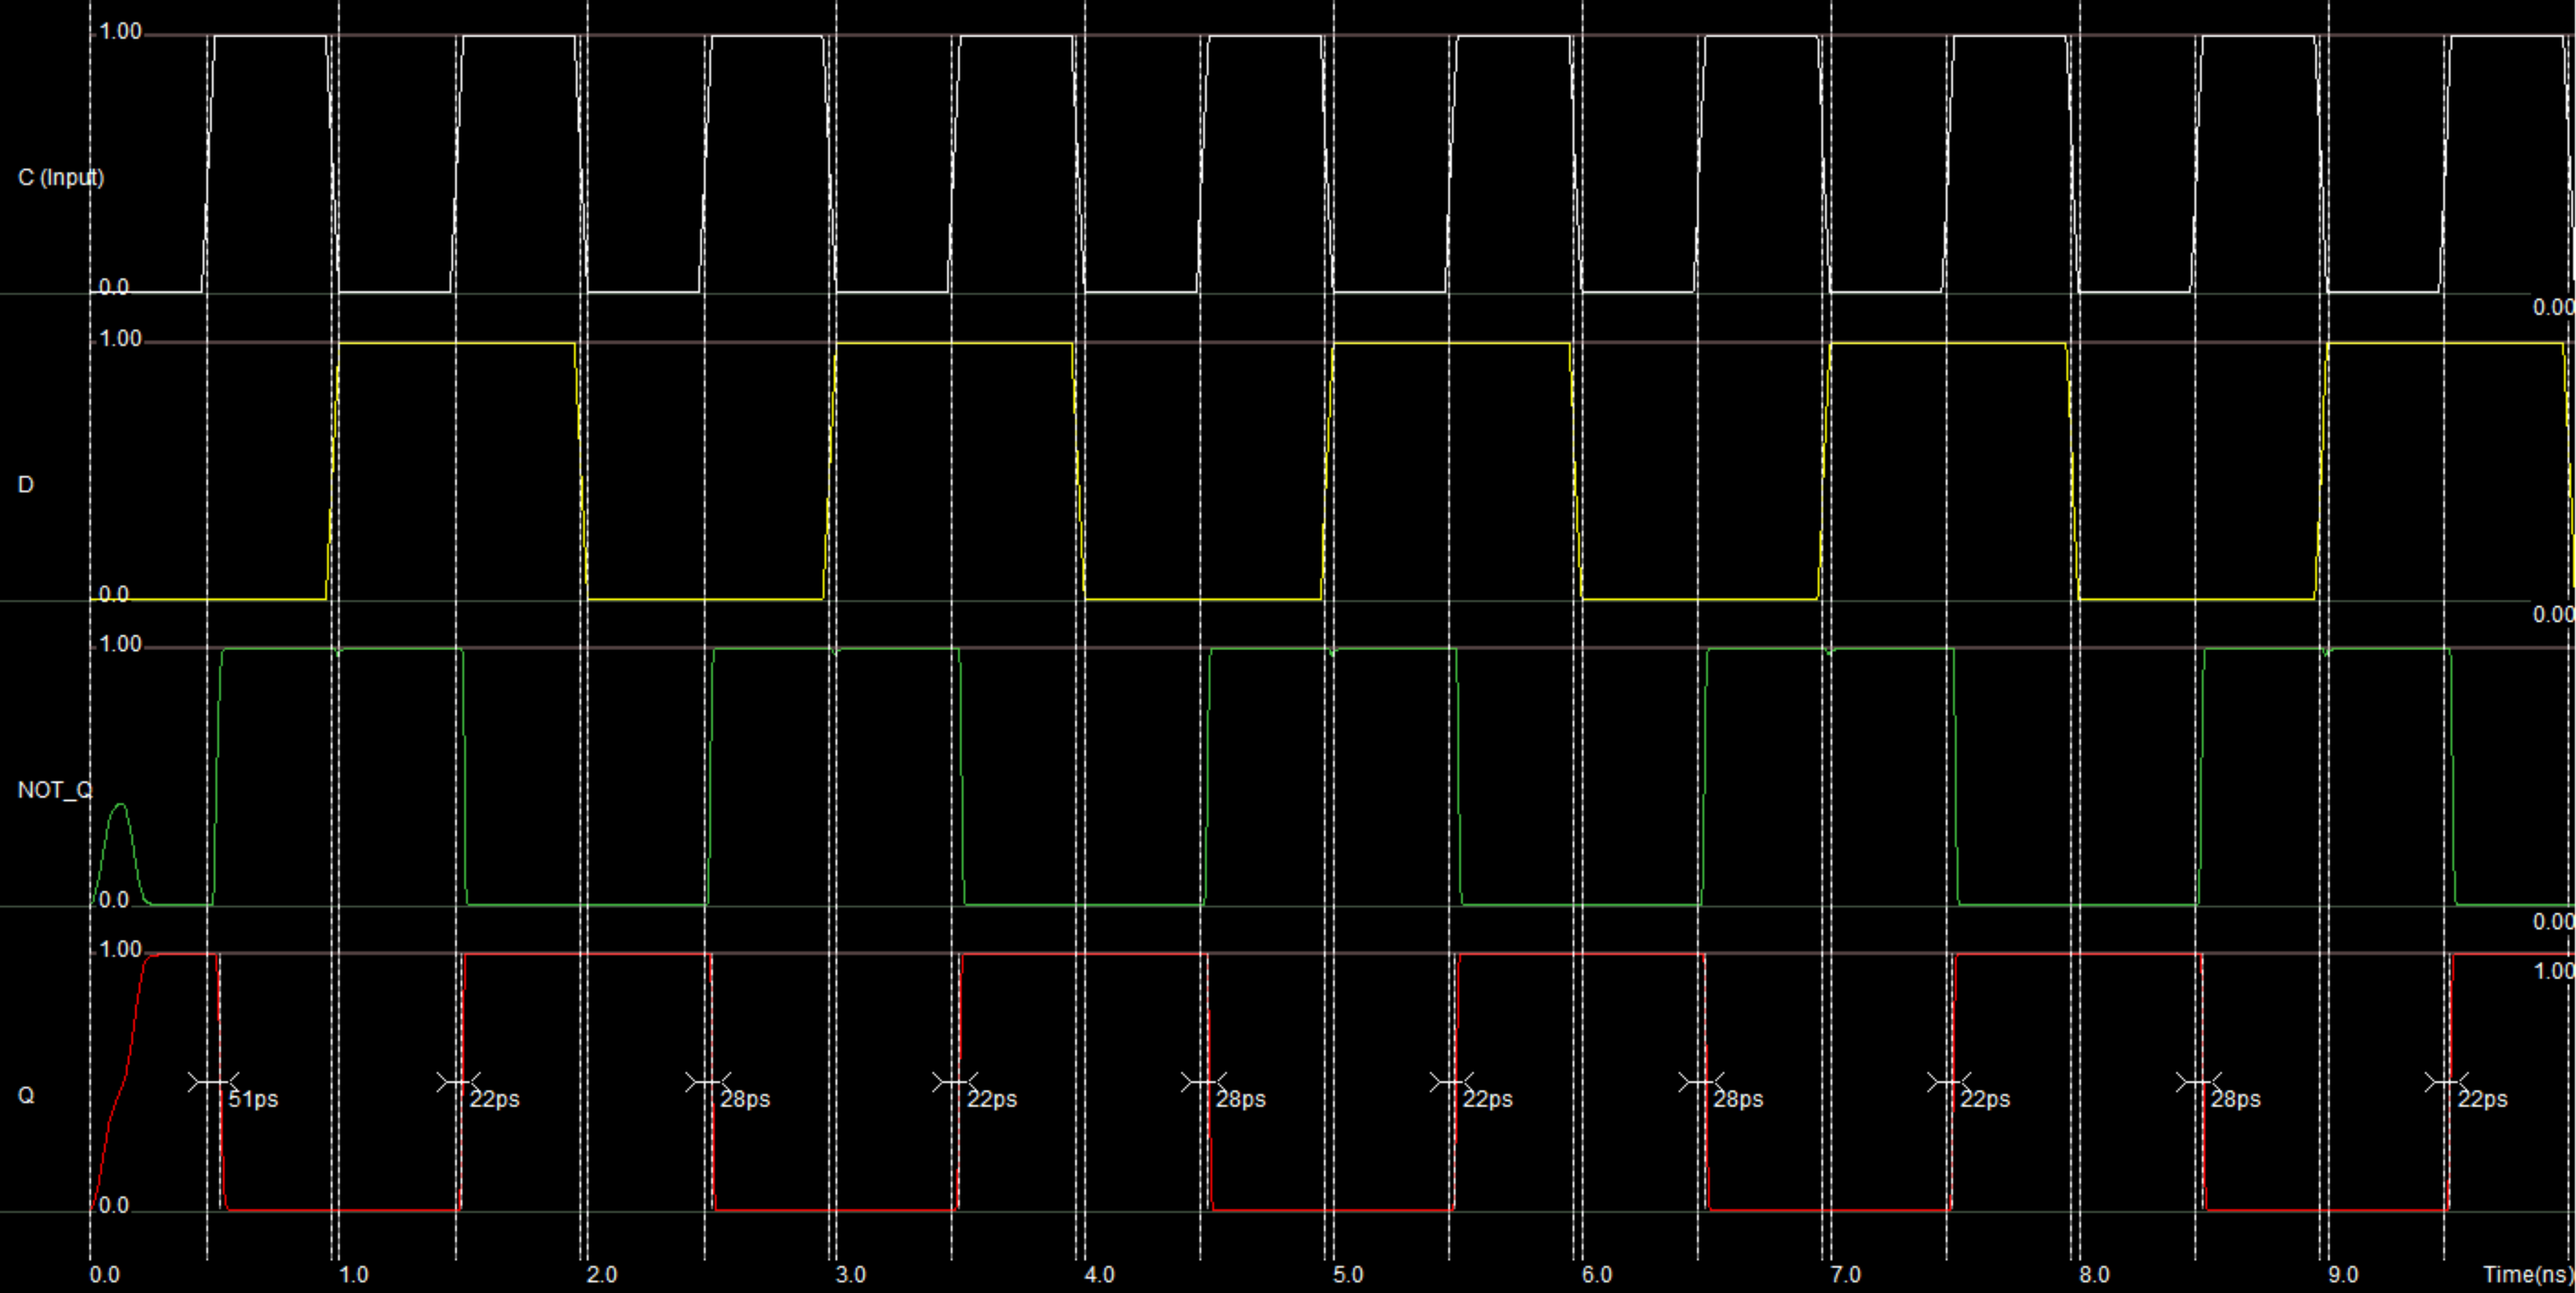
\includegraphics[scale=0.30]{../images/1ghz_test_case_2.PNG}
	\caption{Test Case 2 - $f_C = 1$ \si{\giga\hertz}, Rise/Fall Time $= 0.050$ \si{\nano\second}}
	\label{fig:layout_test_2}
\end{figure}

\FloatBarrier

\begin{figure}[h!]
	\centering
	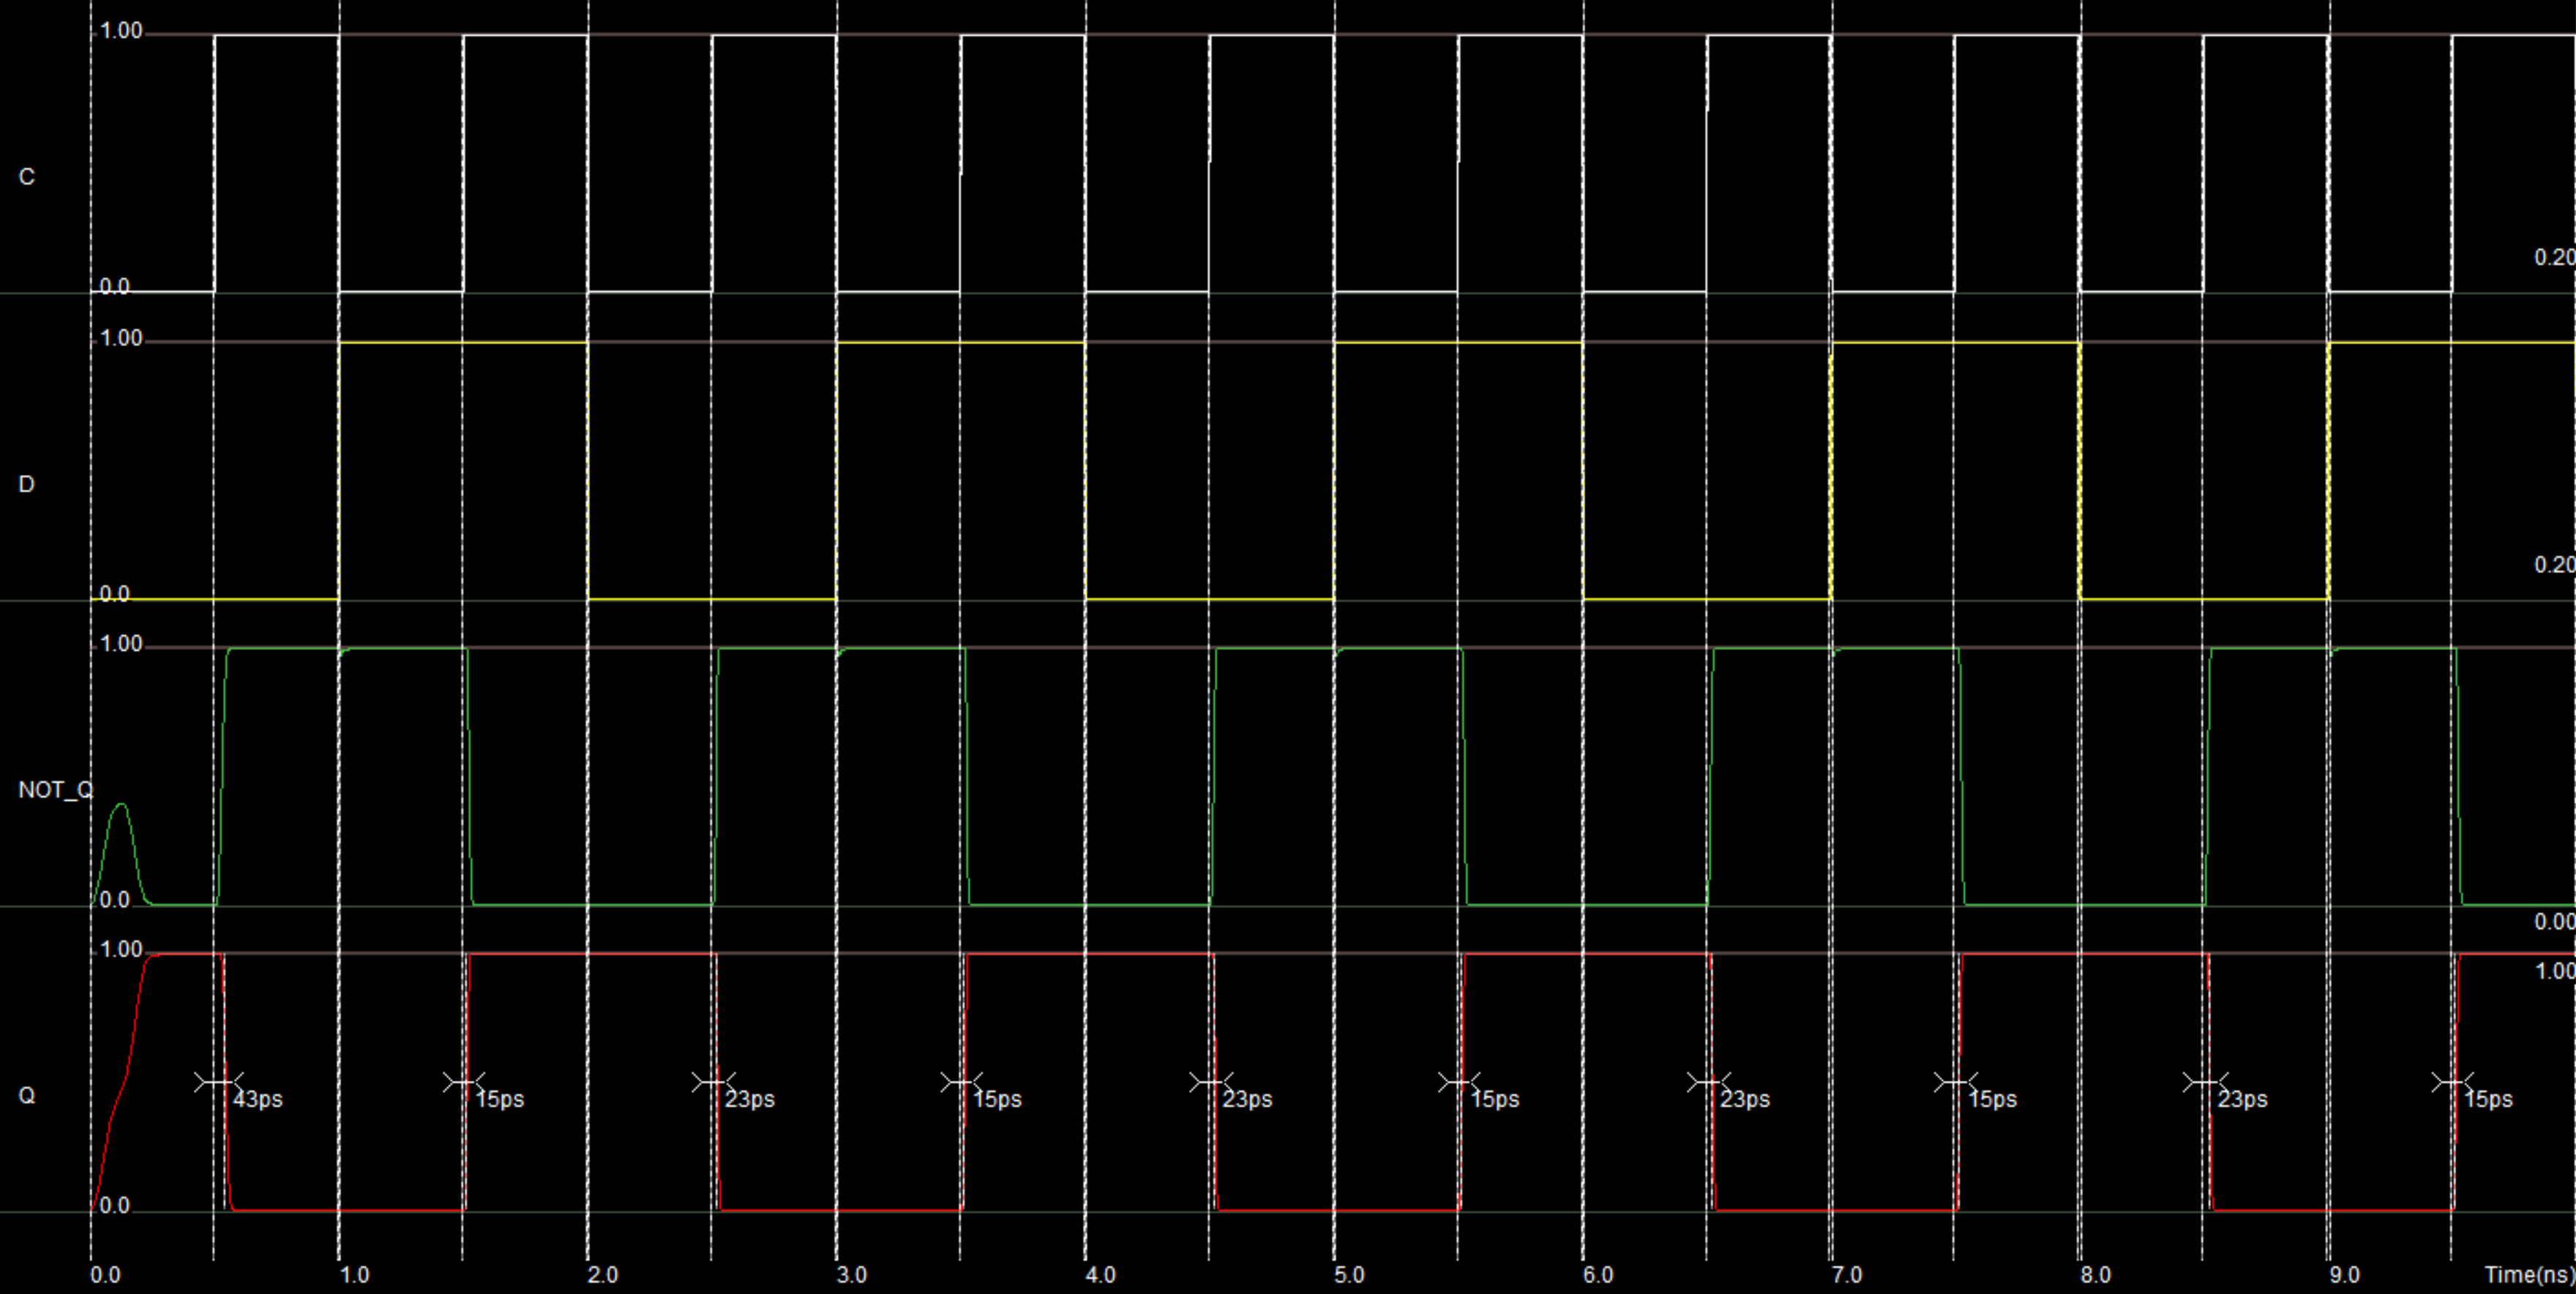
\includegraphics[scale=0.30]{../images/1ghz_test_case_1.PNG}
	\caption{Test Case 3 - $f_C = 1$ \si{\giga\hertz}, Rise/Fall Time $= 0.001$ \si{\nano\second}}
	\label{fig:layout_test_3}
\end{figure}

\FloatBarrier

\begin{figure}[h!]
	\centering
	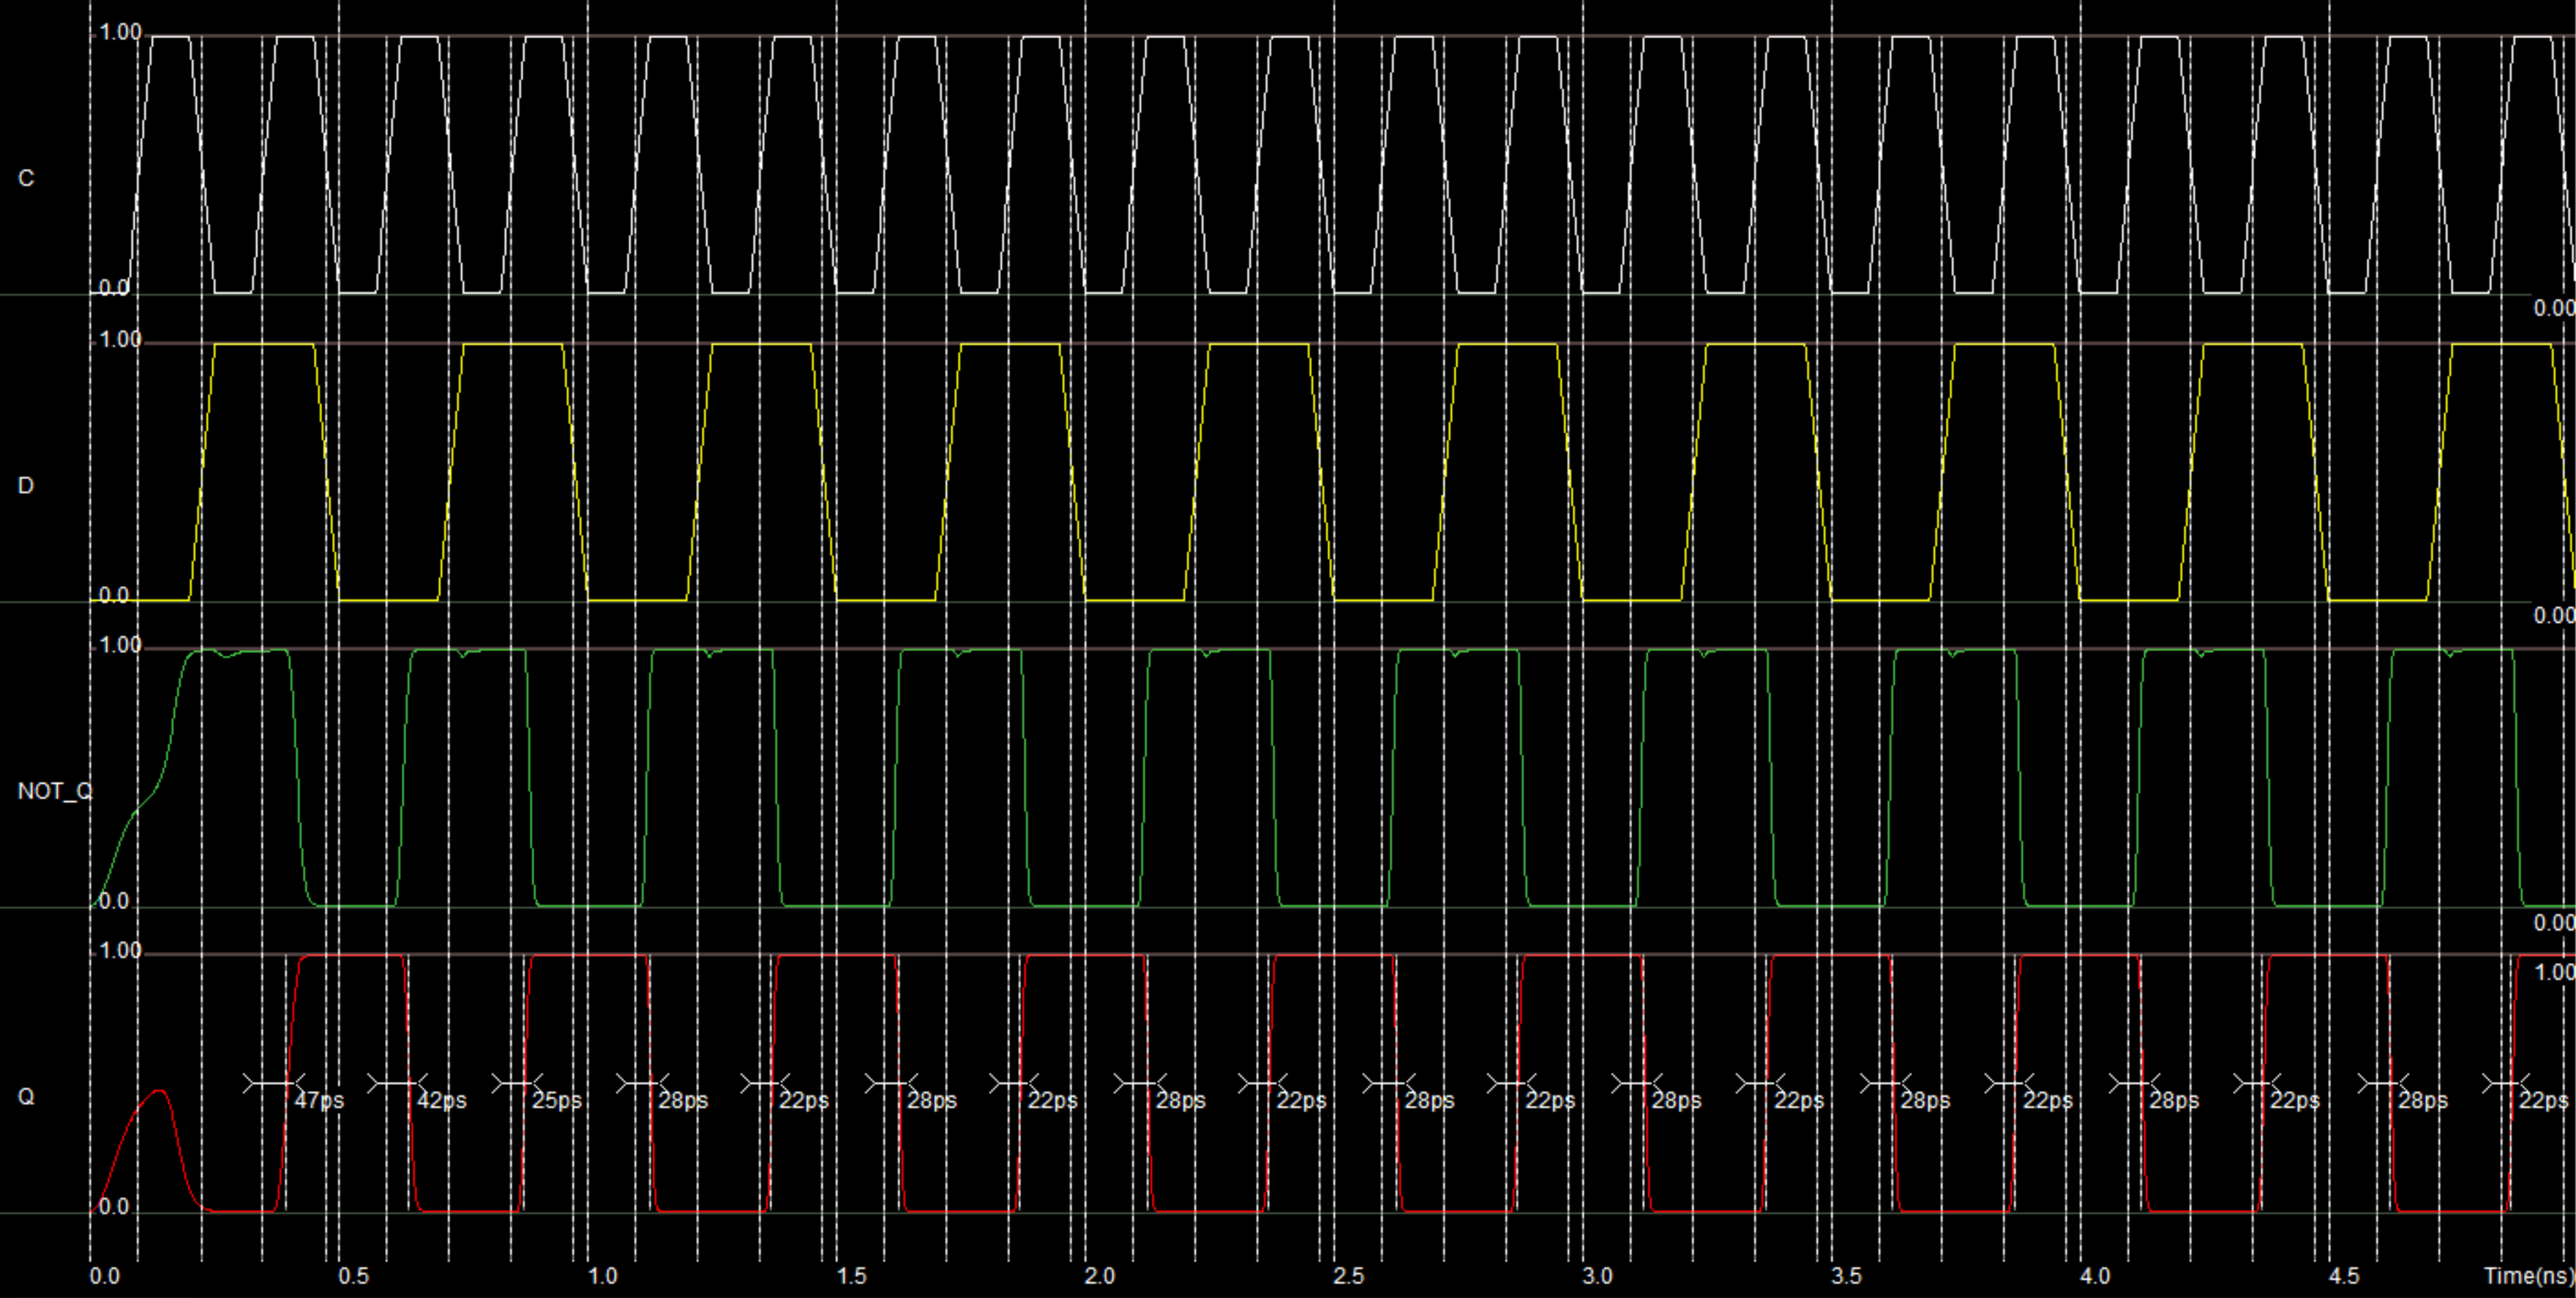
\includegraphics[scale=0.30]{../images/4ghz_test_case_2.PNG}
	\caption{Test Case 4 - $f_C = 4$ \si{\giga\hertz}, Rise/Fall Time $= 0.050$ \si{\nano\second}}
	\label{fig:layout_test_4}
\end{figure}

\FloatBarrier

\begin{figure}[h!]
	\centering
	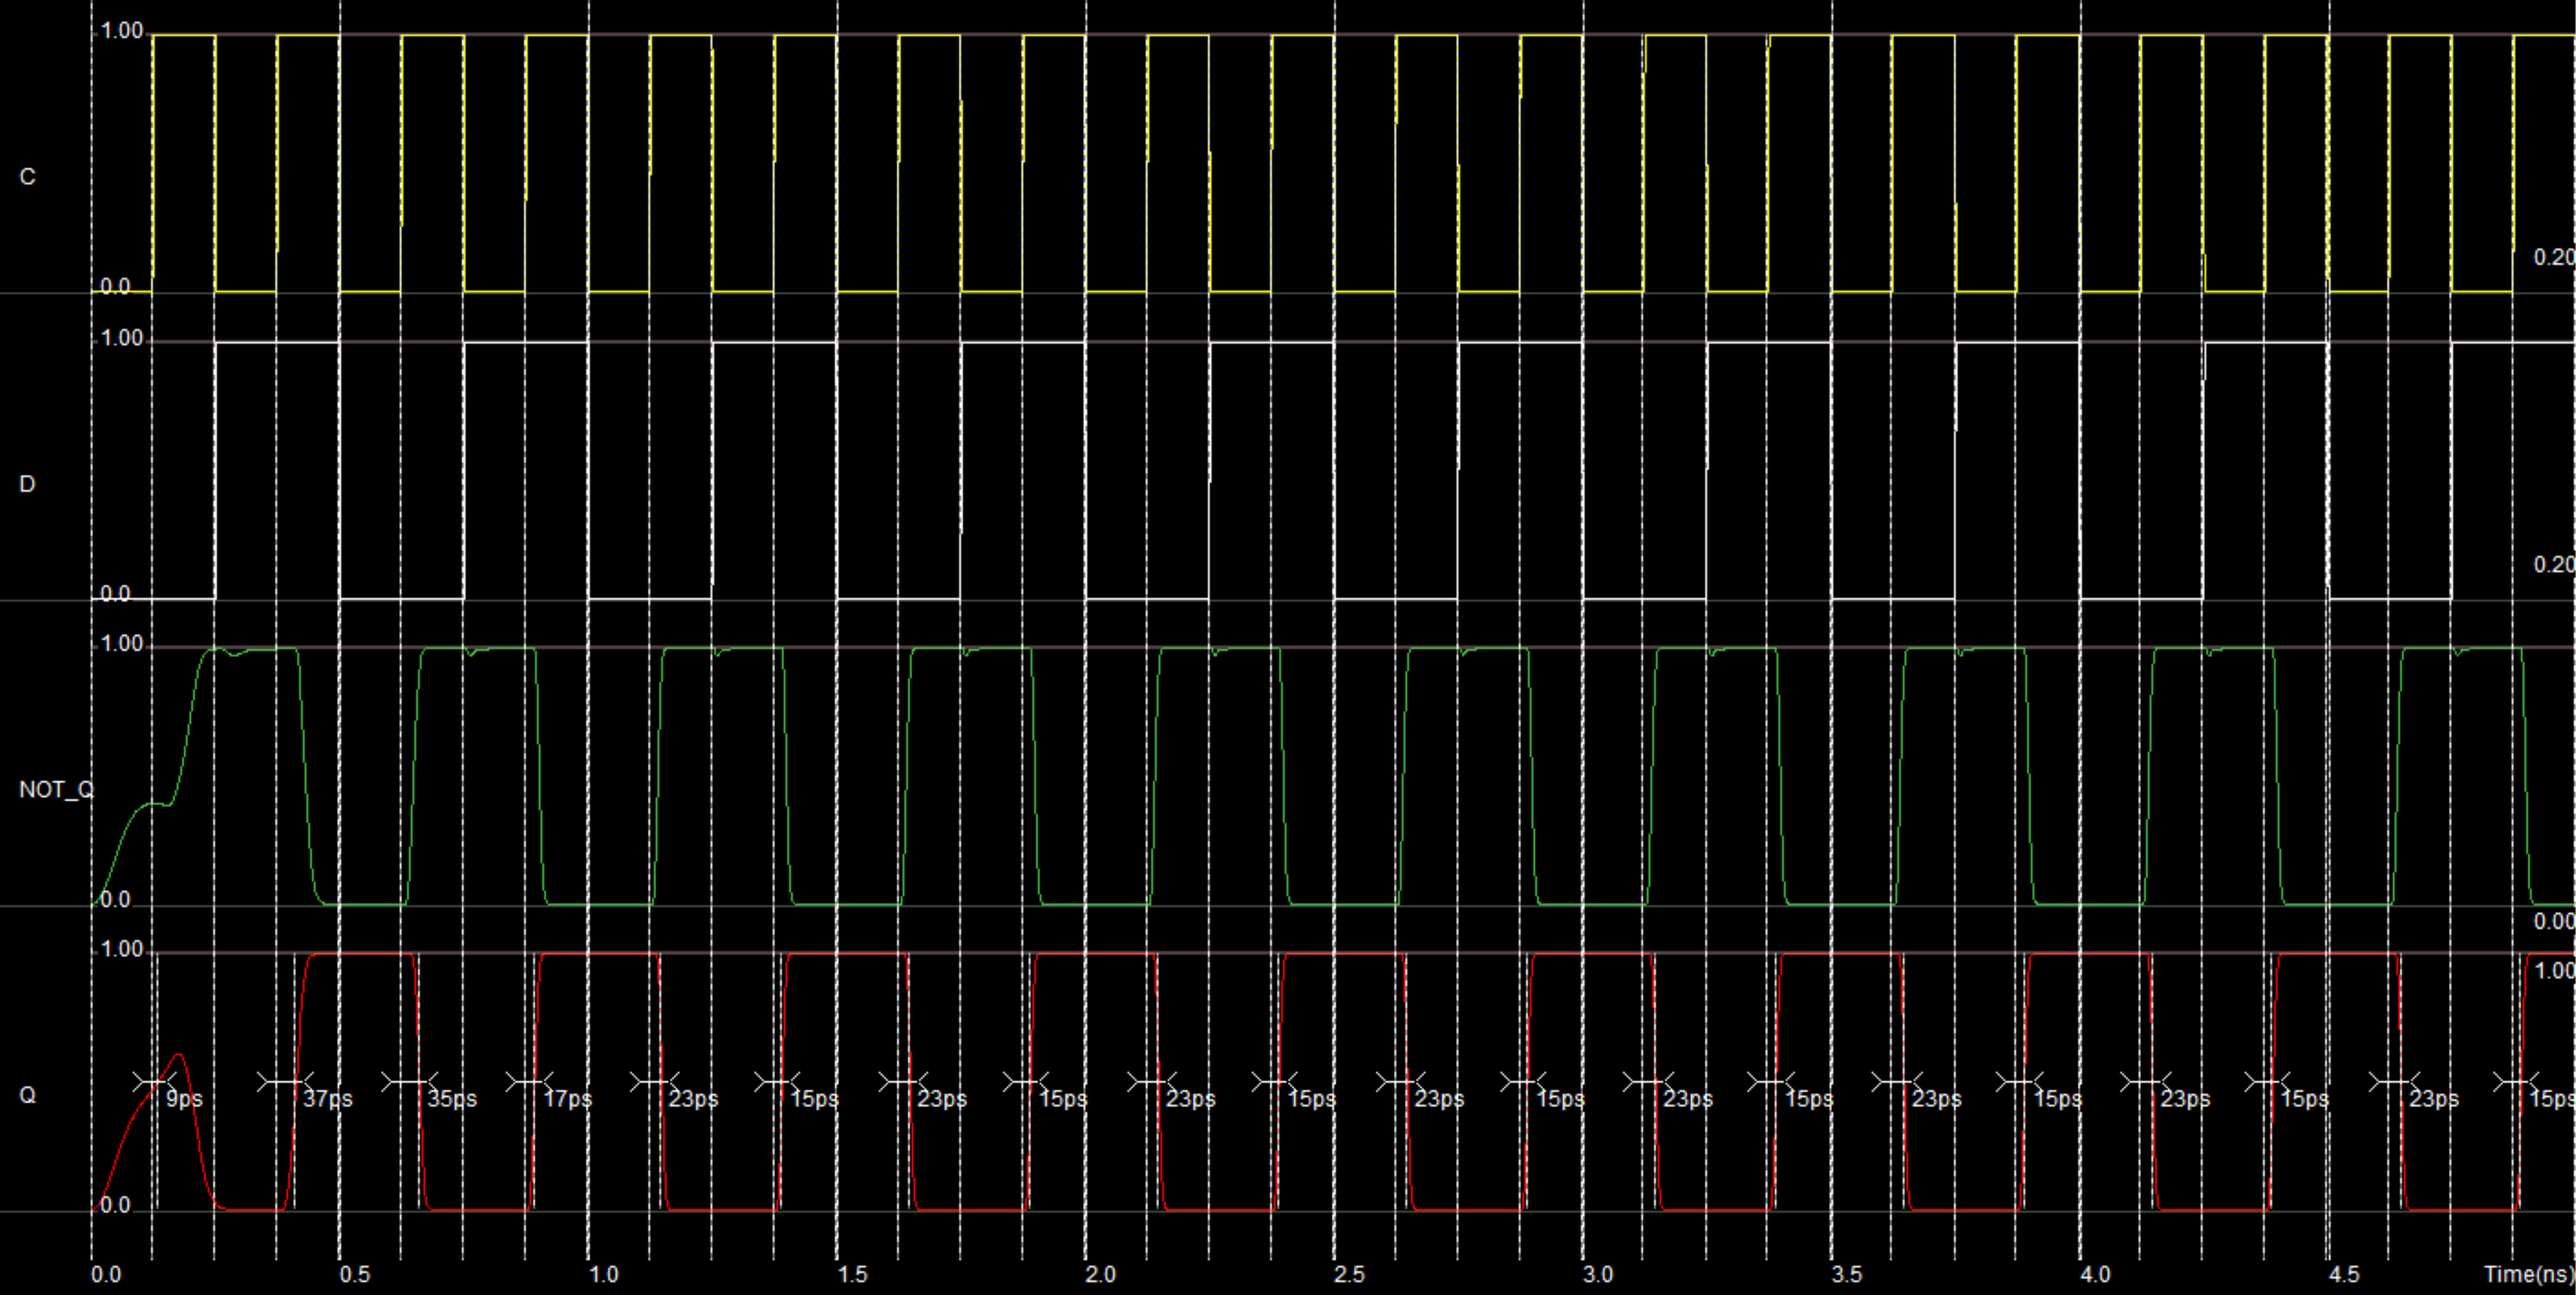
\includegraphics[scale=0.30]{../images/4ghz_test_case_1.PNG}
	\caption{Test Case 5 - $f_C = 4$ \si{\giga\hertz}, Rise/Fall Time $= 0.001$ \si{\nano\second}}
	\label{fig:layout_test_5}
\end{figure}

\FloatBarrier

The following delays and average power dissipation values are found.

\FloatBarrier

\begin{table}[h!]
	\centering
	\caption{D Latch Layout Test Results}
	\label{tab:dlatch_test_results}
	\csvautotabular{../data/dlatch_test_results.csv}
\end{table}

\FloatBarrier

It is observed that the delay of the D Latch is only dependent on the rise and fall times of the input clocks.
This behavior is expected because the dynamic portions of the inputs are kept constant and the length of the static portions of the input should not affect the performance of the circuit as long as they are longer than the delays.

The most ideal rise and fall times of the input clocks, $0.001$ \si{\nano\second}, result in the output delays $\tau_{PHL} = 23$ \si{\pico\second} and $\tau_{PLH} = 15$ \si{\pico\second}.
Taking the longer delay $23$ \si{\pico\second}, the maximum operating frequency of the D Latch is determined to be $1/23$ \si{\pico\second} $= 43$ \si{\giga\hertz}.

The length of the D Latch layout is $12.650$ \si{\micro\meter} and the width of the layout is $5.850$ \si{\micro\meter}. The total area of the layout is $74 \mu m^2$.

\FloatBarrier

\begin{figure}[h!]
	\centering
	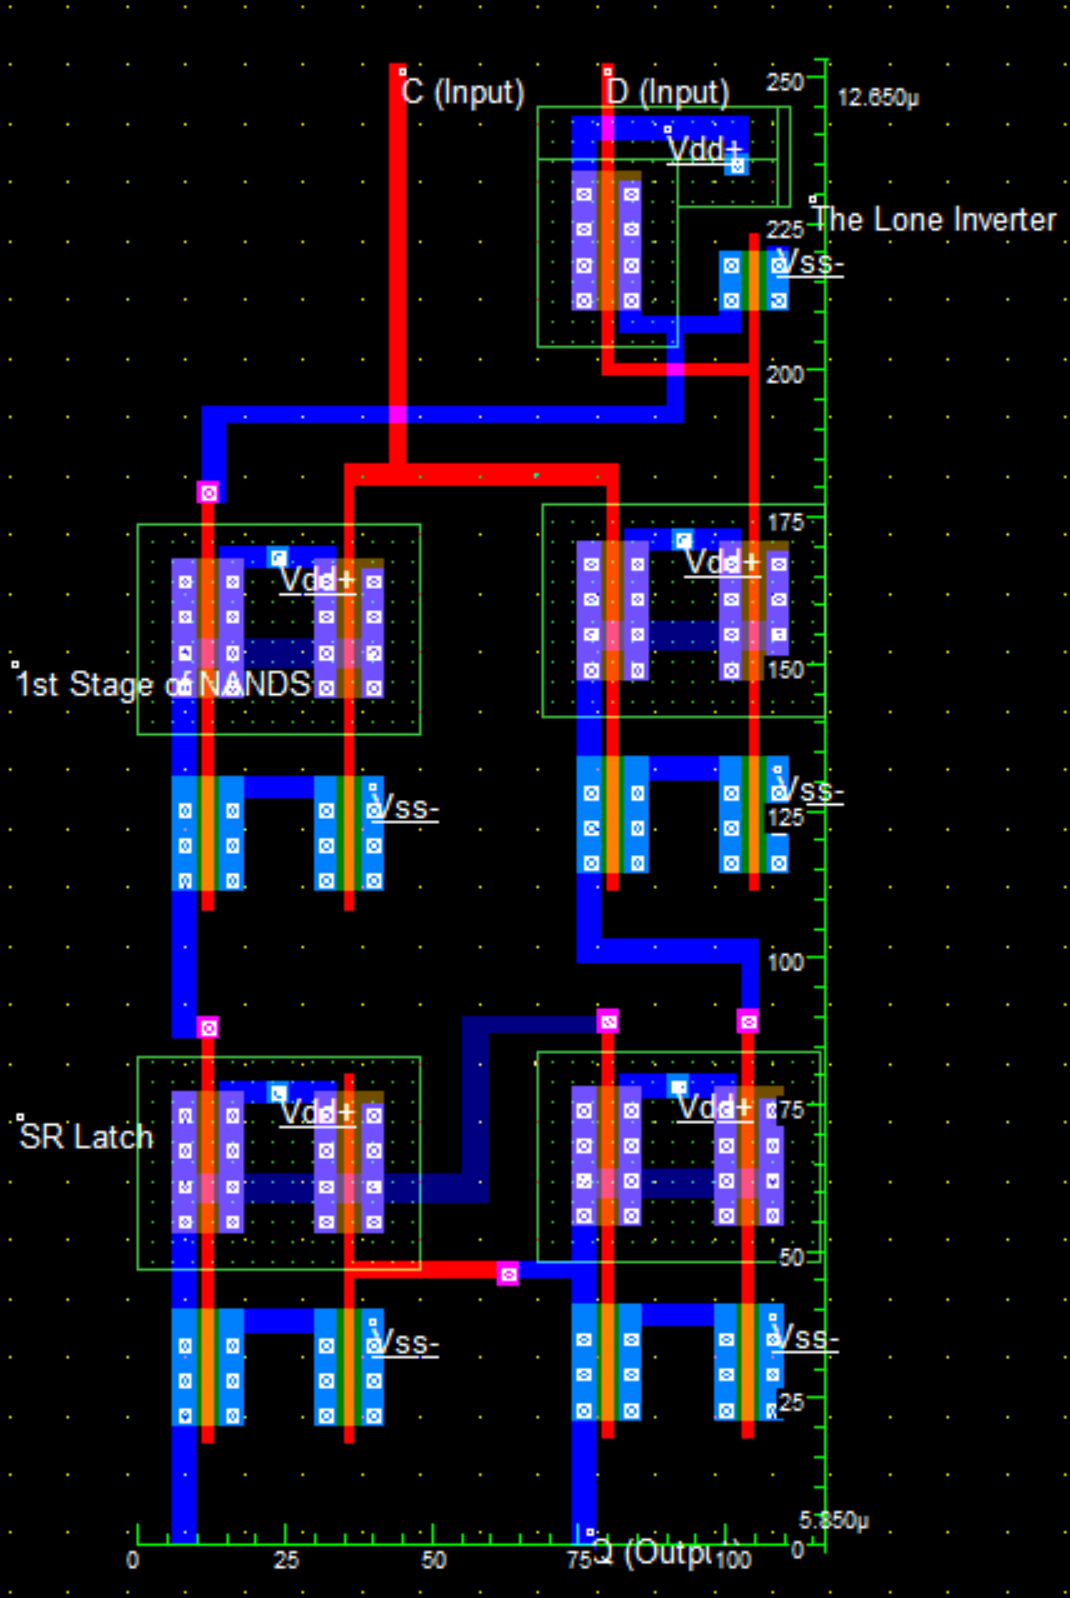
\includegraphics[scale=0.70]{../images/dlatch_layout_area.PNG}
	\caption{Total Area of D Latch Layout}
	\label{fig:dlatch_area}
\end{figure}

\FloatBarrier

Operating at $1$ \si{\giga\hertz}, the average power consumption is determined to be $14.240$ \si{\micro\watt}.
